\definecolor{javared}{rgb}{0.6,0,0} % for strings
\definecolor{javagreen}{rgb}{0.25,0.5,0.35} % comments
\definecolor{javapurple}{rgb}{0.5,0,0.35} % keywords
\definecolor{javadocblue}{rgb}{0.25,0.35,0.75} % javadoc

\lstnewenvironment{code}[1][]%
	{\minipage{\linewidth} 
		\lstset{language=Java,
			basicstyle=\ttfamily,
			keywordstyle=\color{javapurple}\bfseries,
			stringstyle=\color{javared},
			commentstyle=\color{javagreen},
			morecomment=[s][\color{javadocblue}]{/**}{*/},
			numbers=left,
			numberstyle=\tiny\color{black},
			stepnumber=1,
			numbersep=10pt,
			tabsize=4,
			showspaces=false,
			showstringspaces=false}}
	{\endminipage}

\section{NetInfService}
\label{sec:NetInfService}

NetInfService is the first of two Android applications. It provides a NetInf node which can be accessed through a RESTful API. This allows any application running on the same device as the NetInfService to access NetInf functionality through simple HTTP requests. The interface is described in detail in Section \ref{sec:RESTful API}. NetInfService is based on the work done in a previous master thesis \cite{masterthesis} and uses and extends OpenNetInf to provide this functionality. An overview of the design of NetInfService can be seen in Figure \ref{fig:netinfserviceoverview}, the individual components are described below.

\begin{figure}[h!]
	\centering
		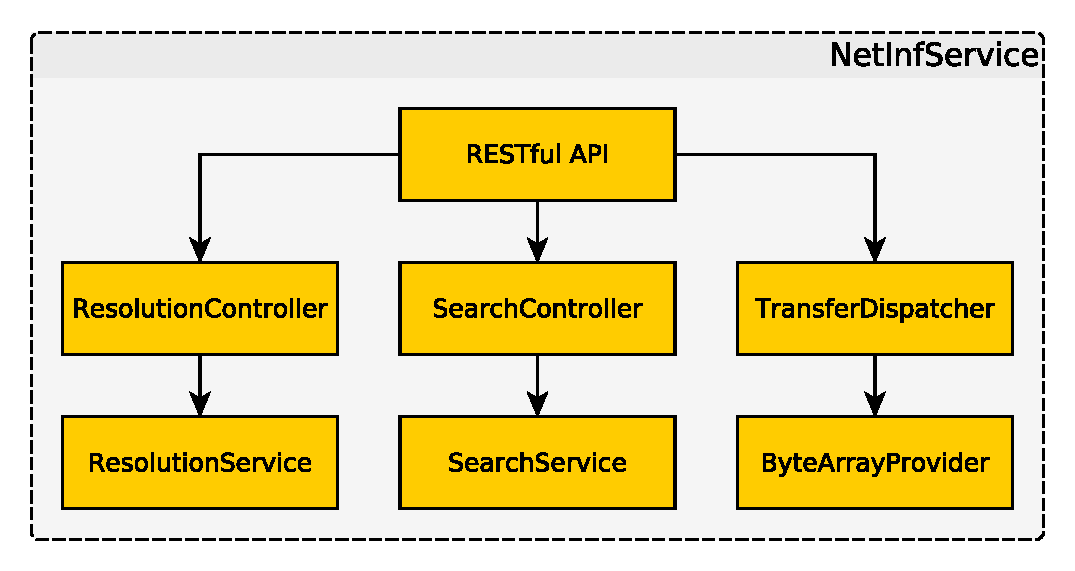
\includegraphics[width=0.75\textwidth]{./img/netinfservice}
    	\caption{NetInfService Overview}
	\label{fig:netinfserviceoverview}
\end{figure}

\subsection{Configuration}
\label{sec:Configuration}

The default settings for NetInfService are stored in the properties file "assets/config.properties". This includes but is not limited to NRS IP address, NRS port and RESTful API port. Some of these settings can be changed live when running the NetInfService on an Android device. This does not change the default values in the properties file but the changes are instead stored using the default Android shared preferences file, which is persistent.

\subsection{RESTful API}
\label{sec:RESTful API}

The RESTful API receives HTTP requests for NetInf functionality. Depending on the type of request, the ResolutionController, SearchController or TransferDispatcher is called. Publish requests are handled by the ResolutionController. Retrieve requests first trigger a get request using the ResolutionController and then, if the get response contained locators, transfer the file using the TransferDispatcher. Search requests are handled by the SearchController.

The HTTP request uses the following format:

\begin{center}
http://\{Host\}:\{Port\}/\{Prefix\}?\{key1\}=\{value1\}\&\{key2\}=\{value2\}...
\end{center}

Since the NetInfService should be running on the same device as the application that is using it, the host would most likely be either localhost or 127.0.0.1. The default port is 8080, for changing it see Section \ref{sec:Configuration}. The key-value pairs should be URL encoded as they can contain illegal characters.

\subsubsection{Publish}

Publish request uses the prefix \emph{publish}.

It requires the following key-value pairs:

\begin{tabular}{ | l | l | }
	\hline
	key & value  \\ \hline \hline
	hash & The hash of the object being published.  \\ \hline
	hashAlg & The hash algorithm used to hash the object. \\ \hline
	ct & The MIME content-type of the object being published. \\ \hline
\end{tabular}

The following key-value pairs are optional:

\begin{tabular}{ | l | l | }
	\hline
	key & value  \\ \hline \hline
	btmac & The Bluetooth MAC address of the publishing device. \\ \hline
	meta & Metadata as a JSON string. \\ \hline
	filepath & Path to the file being publish. \\ \hline
\end{tabular}

\begin{itemize}
	\item btmac: The Bluetooth MAC address of the publishing device, it will be added as a locator to the published object.
	\item meta: The metadata of the object that is being published. Remember to URL encode illegal characters.
	\item filepath: The file path of the object that is being published. If this is present, a full put is done, otherwise not.
 \end{itemize}

A successful publish returns HTTP status code 200. Any other code indicates that something went wrong and should give an indication of what went wrong.

Below is an example of how a HTTP publish request could look like, notice the URL encoding:

http://localhost:8080/publish?hash=TcoP1fQkoxsDq4B8uud\%2Bsyvy0Inu0c7hVLOv7UWN4Nw \\ \&hashAlg=sha-256\&ct=text\%2Fplain\&btmac=F0\%3AE7\%3A7E\%3A3F\%3AD2\%3A43

Unencoded it would look like:

http://localhost:8080/publish?hash=TcoP1fQkoxsDq4B8uud+syvy0Inu0c7hVLOv7UWN4Nw \\ \&hashAlg=sha-256\&ct=text/plain\&btmac=F0:E7:7E:3F:D2:43

\subsection{Retrieve}

Retrieve requests use the prefix \emph{retrieve}.

It requires the following key-value pairs:

\begin{tabular}{ | l | l | }
	\hline
	key & value  \\ \hline \hline
	hash & The hash of the object being published.  \\ \hline
	hashAlg & The hash algorithm used to hash the object. \\ \hline
\end{tabular}

A successful retrieve returns HTTP status code 200. The HTTP response should contain a JSON object with two key-value pairs. The key \emph{path} should contain a local file path to the retrieved object. The key \emph{ct} should contain the MIME content-type of the retrieved object. Any other code indicates that something went wrong and should give an indication of what went wrong.

Below is an example of how a HTTP retrieve request could look like, notice the URL encoding:

http://localhost:8080/retrieve?hash=TcoP1fQkoxsDq4B8uud\%2Bsyvy0Inu0c7hVLOv7UWN4Nw \\ \&hashAlg=sha-256

Unencoded it would look like:

http://localhost:8080/retrieve?hash=TcoP1fQkoxsDq4B8uud+syvy0Inu0c7hVLOv7UWN4Nw \\ \&hashAlg=sha-256

\subsection{Search}

Search requests use the prefix \emph{search}.

It requires the following key-value pairs:

\begin{tabular}{ | l | l | }
	\hline
	key & value  \\ \hline \hline
	tokens & The tokens being searched for.  \\ \hline
\end{tabular}

The following key-value pair is optional:

\begin{tabular}{ | l | l | }
	\hline
	key & value  \\ \hline \hline
	ext & An optional JSON, meant for future extensions. \\ \hline
\end{tabular}

\begin{itemize}
	\item tokens: Currently NetInfService only supports one token. This should be changed to accept a string of space separated search tokens to follow specification.
	\item ext: The ext field is meant for future extensions. It is allowed, but currently ignored.
 \end{itemize}

Below is an example of how a HTTP search request could look like, notice the URL encoding:

http://localhost:8080/search?tokens=http\%3A\%2F\%2Fwww.ericsson.com\%2F

Unencoded it would look like:

http://localhost:8080/search?tokens=http://www.ericsson.com/

\subsection{ResolutionController}
\label{sec:ResolutionController}

The ResolutionController handles a number of ResolutionServices. Each ResolutionService should provide publish, get, and delete functionality using some convergence layer or equivalent. Currently there are two ResolutionServices, the LocalResolutionService which uses a local SQLite database and the NameResolutionService which communicates with a specific NRS using the HTTP convergence layer.

\subsubsection{NameResolutionService}

The NameResolutionService uses the HTTP convergence layer (TODO REFS) to communicate with a single NRS. Currently the NameResolutionService supports publish and get. Delete is not yet supported but the framework for its implementation is there so it should be relatively little work.

\subsubsection{LocalResolutionService}

The LocalResolutionService uses a to the device local SQLite database. The LocalResolutionService has higher priority than the NameResolutionService meaning that when preforming a get request the LocalResolutionService will be used first and then if needed the NameResolutionService as well.

\subsection{SearchController}
\label{sec:SearchController}

The SearchController handles a number of SearchServices. Each SearchService should provide search functionality 
using some convergence layer or equivalent. Currently there is one SearchService, the UrlSearchService, 
which provides search functionality using a single token which is assumed to be a URL.

\subsubsection{UrlSearchService}

The UrlSearchService provides the functionality to search for a single token in the local database 
used by the LocalResolutionService and then, if not found, using the HTTP convergence layer to search 
in the NRS used by the NameResolutionService.

\subsection{TransferDispatcher}
\label{sec:TransferDispatcher}

The TransferDispatcher handles a number of ByteArrayProviders. Each ByteArrayProvider should provide functionality to retrieve a file (as a byte array) in some way. Currently there is one ByteArrayProvider, the BluetoothProvider, which uses Bluetooth to transfer files between Bluetooth enabled devices.

\subsubsection{BluetoothProvider}
The BluetoothProvider provides the functionality to retrieve the bytes of an Information Object
through a specified Bluetooth locator. It first tries to establish a connection to the remote
Bluetooth device. If successful, it requests the bytes of an object by sending the hash value
that describes the object. As a response, the provider retrieves the bytes of the object, if
it was available on the remote Bluetooth device.

\subsubsection{BluetoothServer}
The BluetoothServer continuously listens to incoming Bluetooth file requests. 
If a remote device wants to connect to the local device, the BluetoothServer establishes
a BluetoothSocket through which both devices can communicate with each other.
The BluetoothServer expects to receive a string that represents a hash
of a requested object. Using this hash, the BluetoothServer will send back
the byte arrays of the corresponding object, if available. 

\section{Elephant}
\label{sec:Elephant}

Elephant is the second Android application. It is a simple browser which uses NetInf through the NetInfService to cache and share web pages.

The idea behind the Elephant browser is simple. When a traditional web URL is entered into the address bar and the refresh button is clicked, instead of just downloading the web page from the Internet the browser first tries to use NetInf to retrieve the web page.

This is done by using the NetInfService. For the entered URL and each resource it links to:
\begin{enumerate}
	\item Search for the hash of the URL/resource.
	\item Get the file with the given hash.
	\item Possibly publish the file so that other devices can retrieve the file from this device.
\end{enumerate}

If the search or get fails for any reason, be it a timeout, no matches found or something else, the webpage is downloaded using the Internet.

\subsection{Configuration}

The default settings for Elephant are stored in the properties file "assets/config.properties". This includes but is not limited to RESTful API IP address, RESTful API port and RESTful API timeouts.

\subsection{Control Flow}
\label{sec:Control Flow}

Figure \ref{fig:macro-controlflow} shows an overview of the control flow of the interaction between Elephant and NetInfService.
Figure \ref{fig:application-controlflow} shows a picture of the internal control flow of the Elephant web browser.
Figure \ref{fig:netinf-controlflow} shows a picture of the internal control flow of the NetInf service.

Pictures \ref{fig:application-controlflow} and \ref{fig:netinf-controlflow} provides the packages and/or source files that are
involved in different parts of the program, as well as some text and arrows describing the control flow.

The NetInfService mainly does its work by passing around Identifiers and InformationObjects (each encapsulating an Identifier).

An Identifier contains information about an InformationObject. The most important pieces of information in these applications are:
\begin{itemize}
\item Hash Algorithm
\item Hash
\item Content-Type
\item Metadata (as a JSON string)
\end{itemize}

InformationObjects can contain attributes. In these applications the only used attributes are locator attributes. More specifically locators pointing to other Bluetooth devices and locators pointing to the local file system.

\begin{figure}
\centering
\centerline{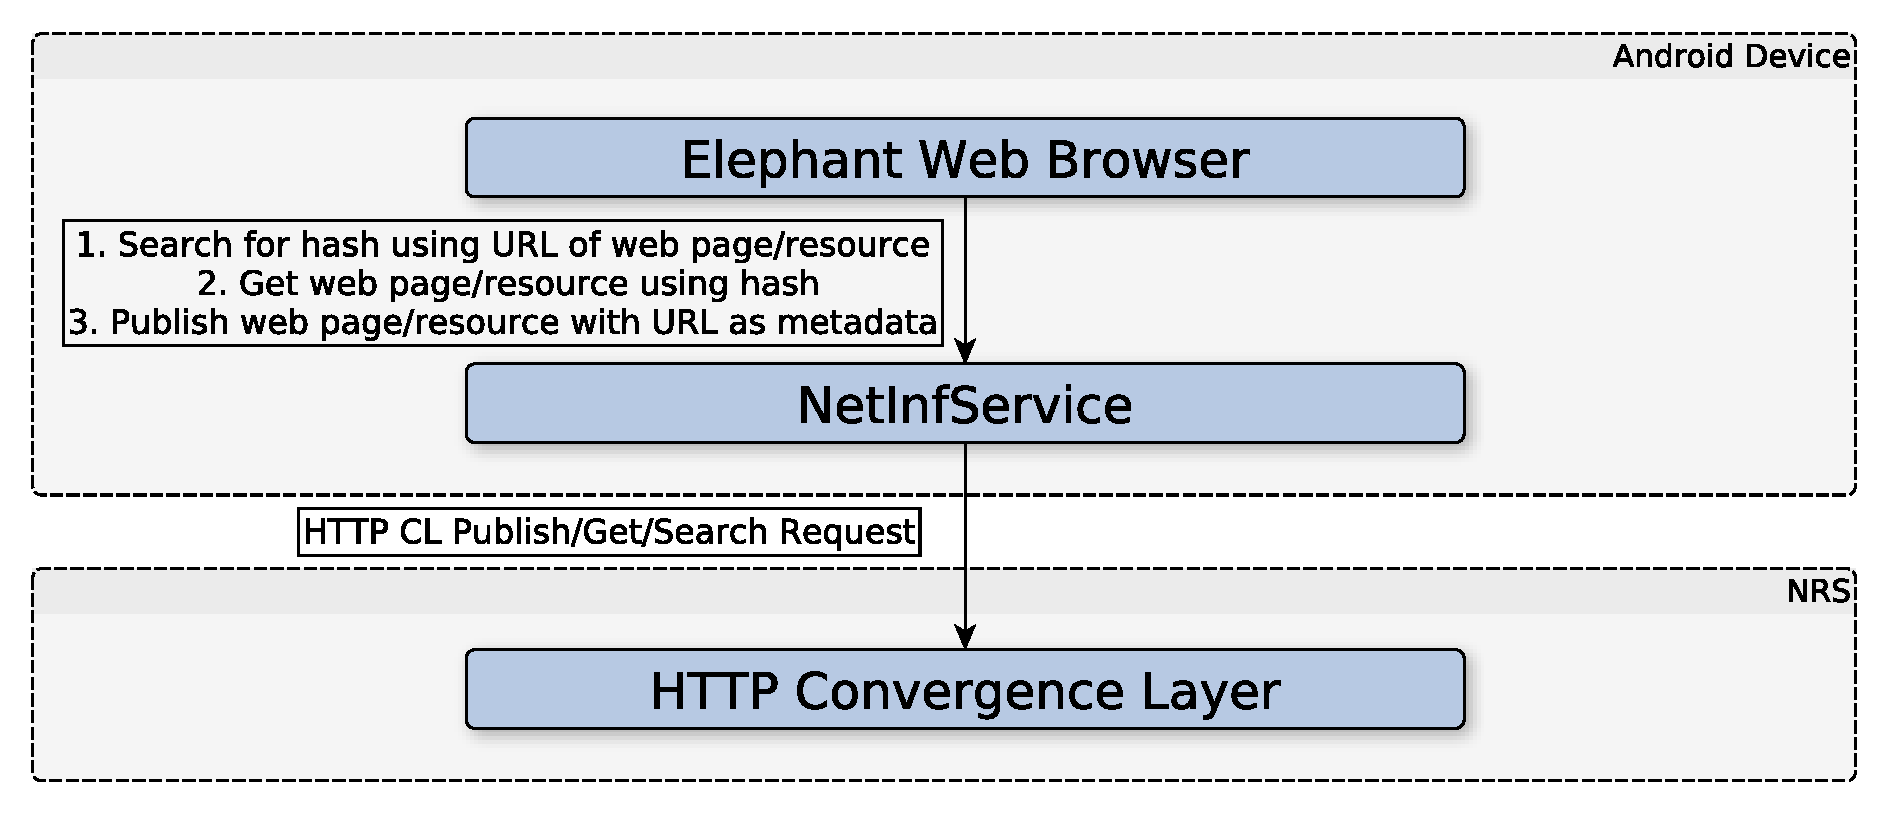
\includegraphics[width=1.4\textwidth]{./img/flowchart-macros.pdf}}
\caption{Elephant/NetInfService Control Flow}
\label{fig:macro-controlflow}
\end{figure}

\begin{figure}
\centering
\centerline{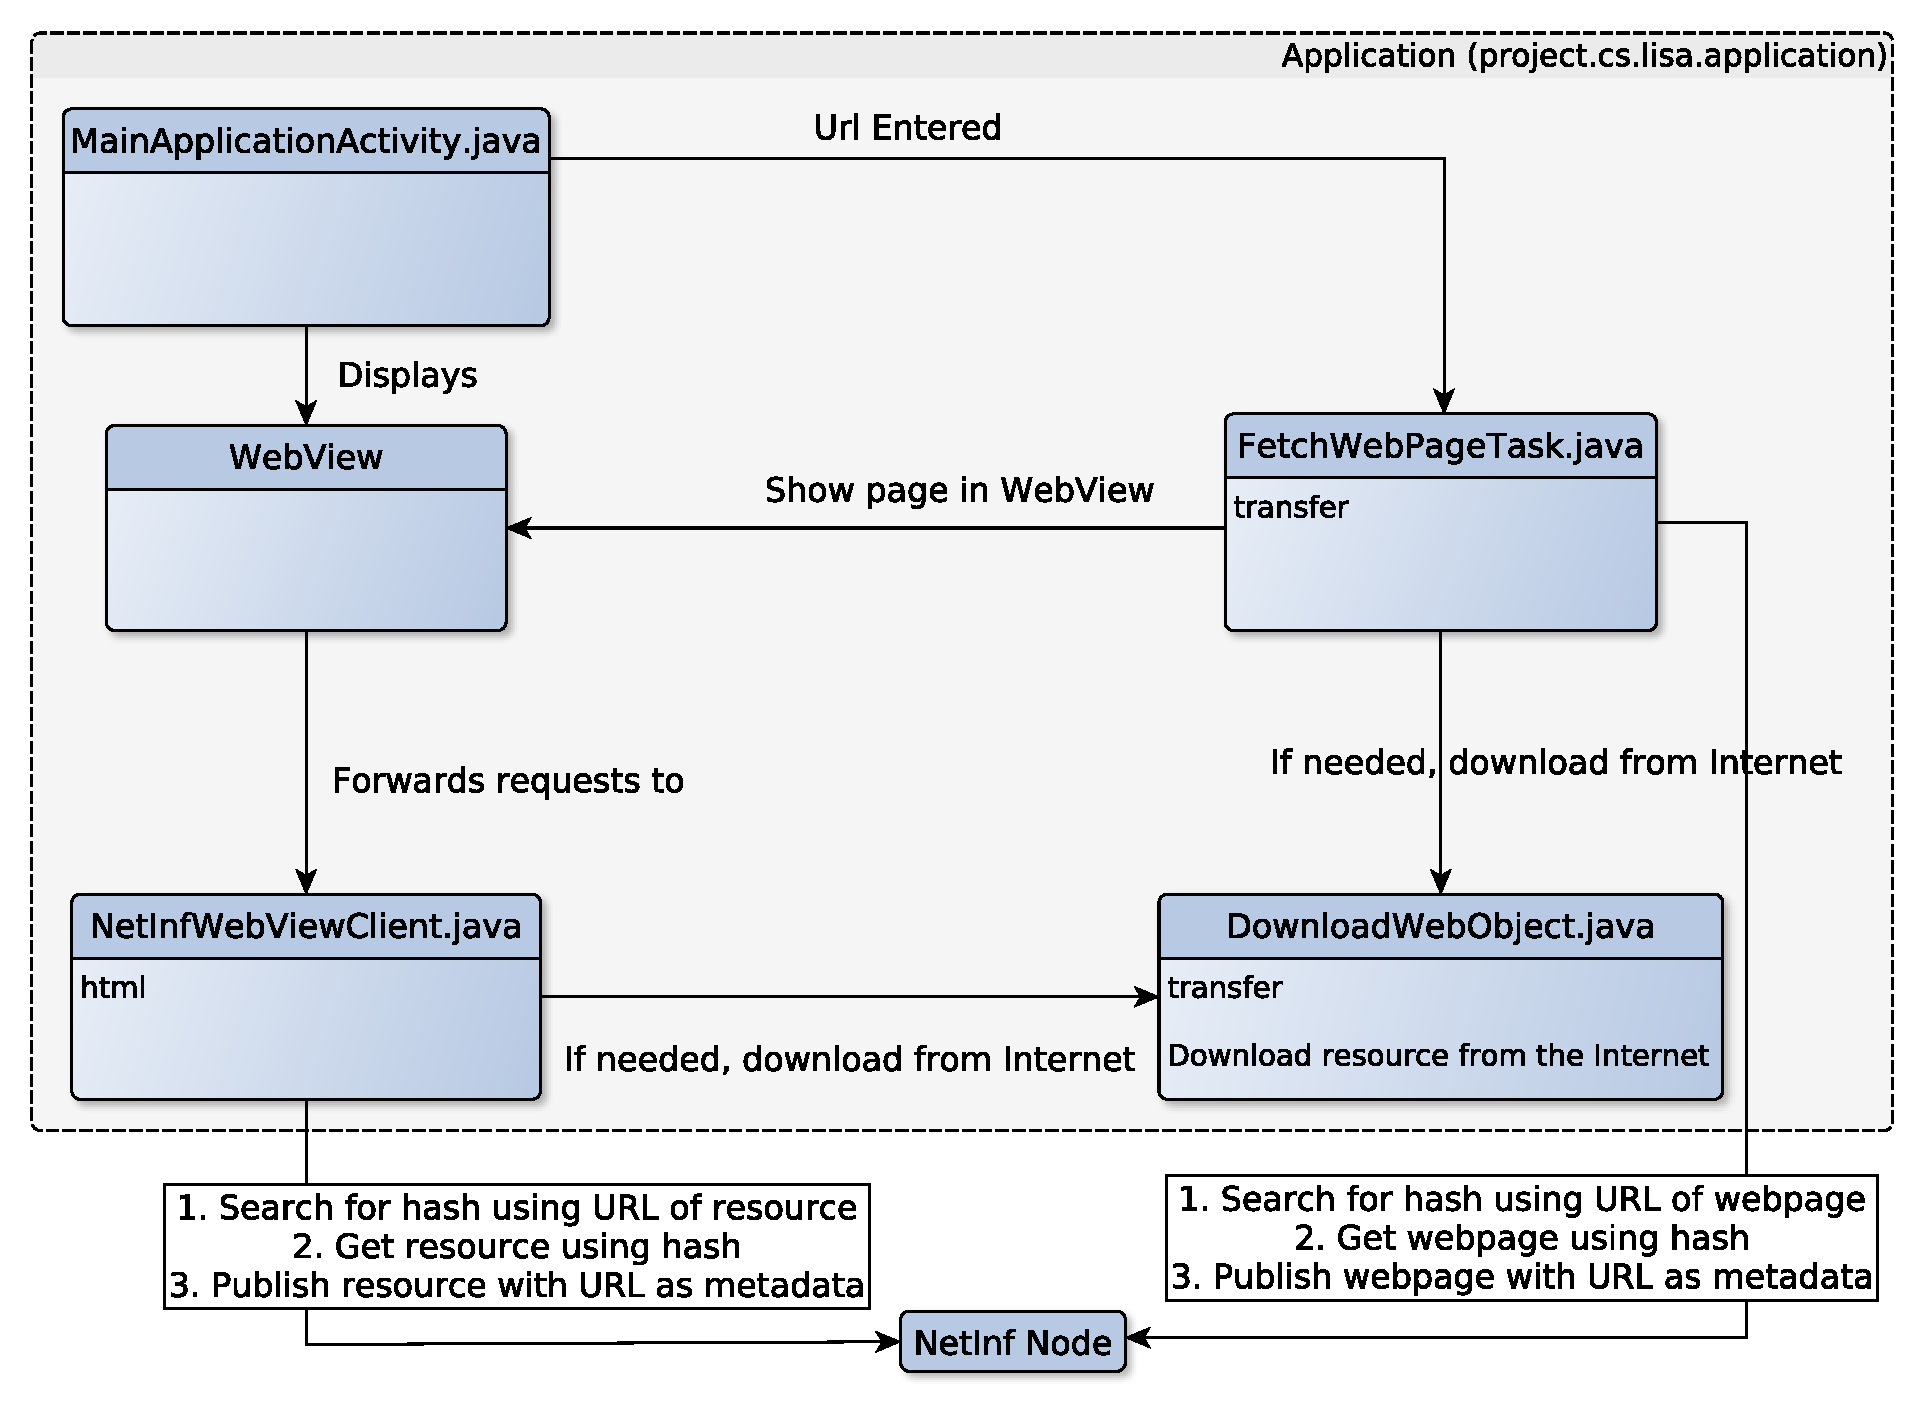
\includegraphics[width=1.4\textwidth]{./img/flowchart-application.pdf}}
\caption{Elephant Control Flow}
\label{fig:application-controlflow}
\end{figure}

\begin{figure}
\centering
\centerline{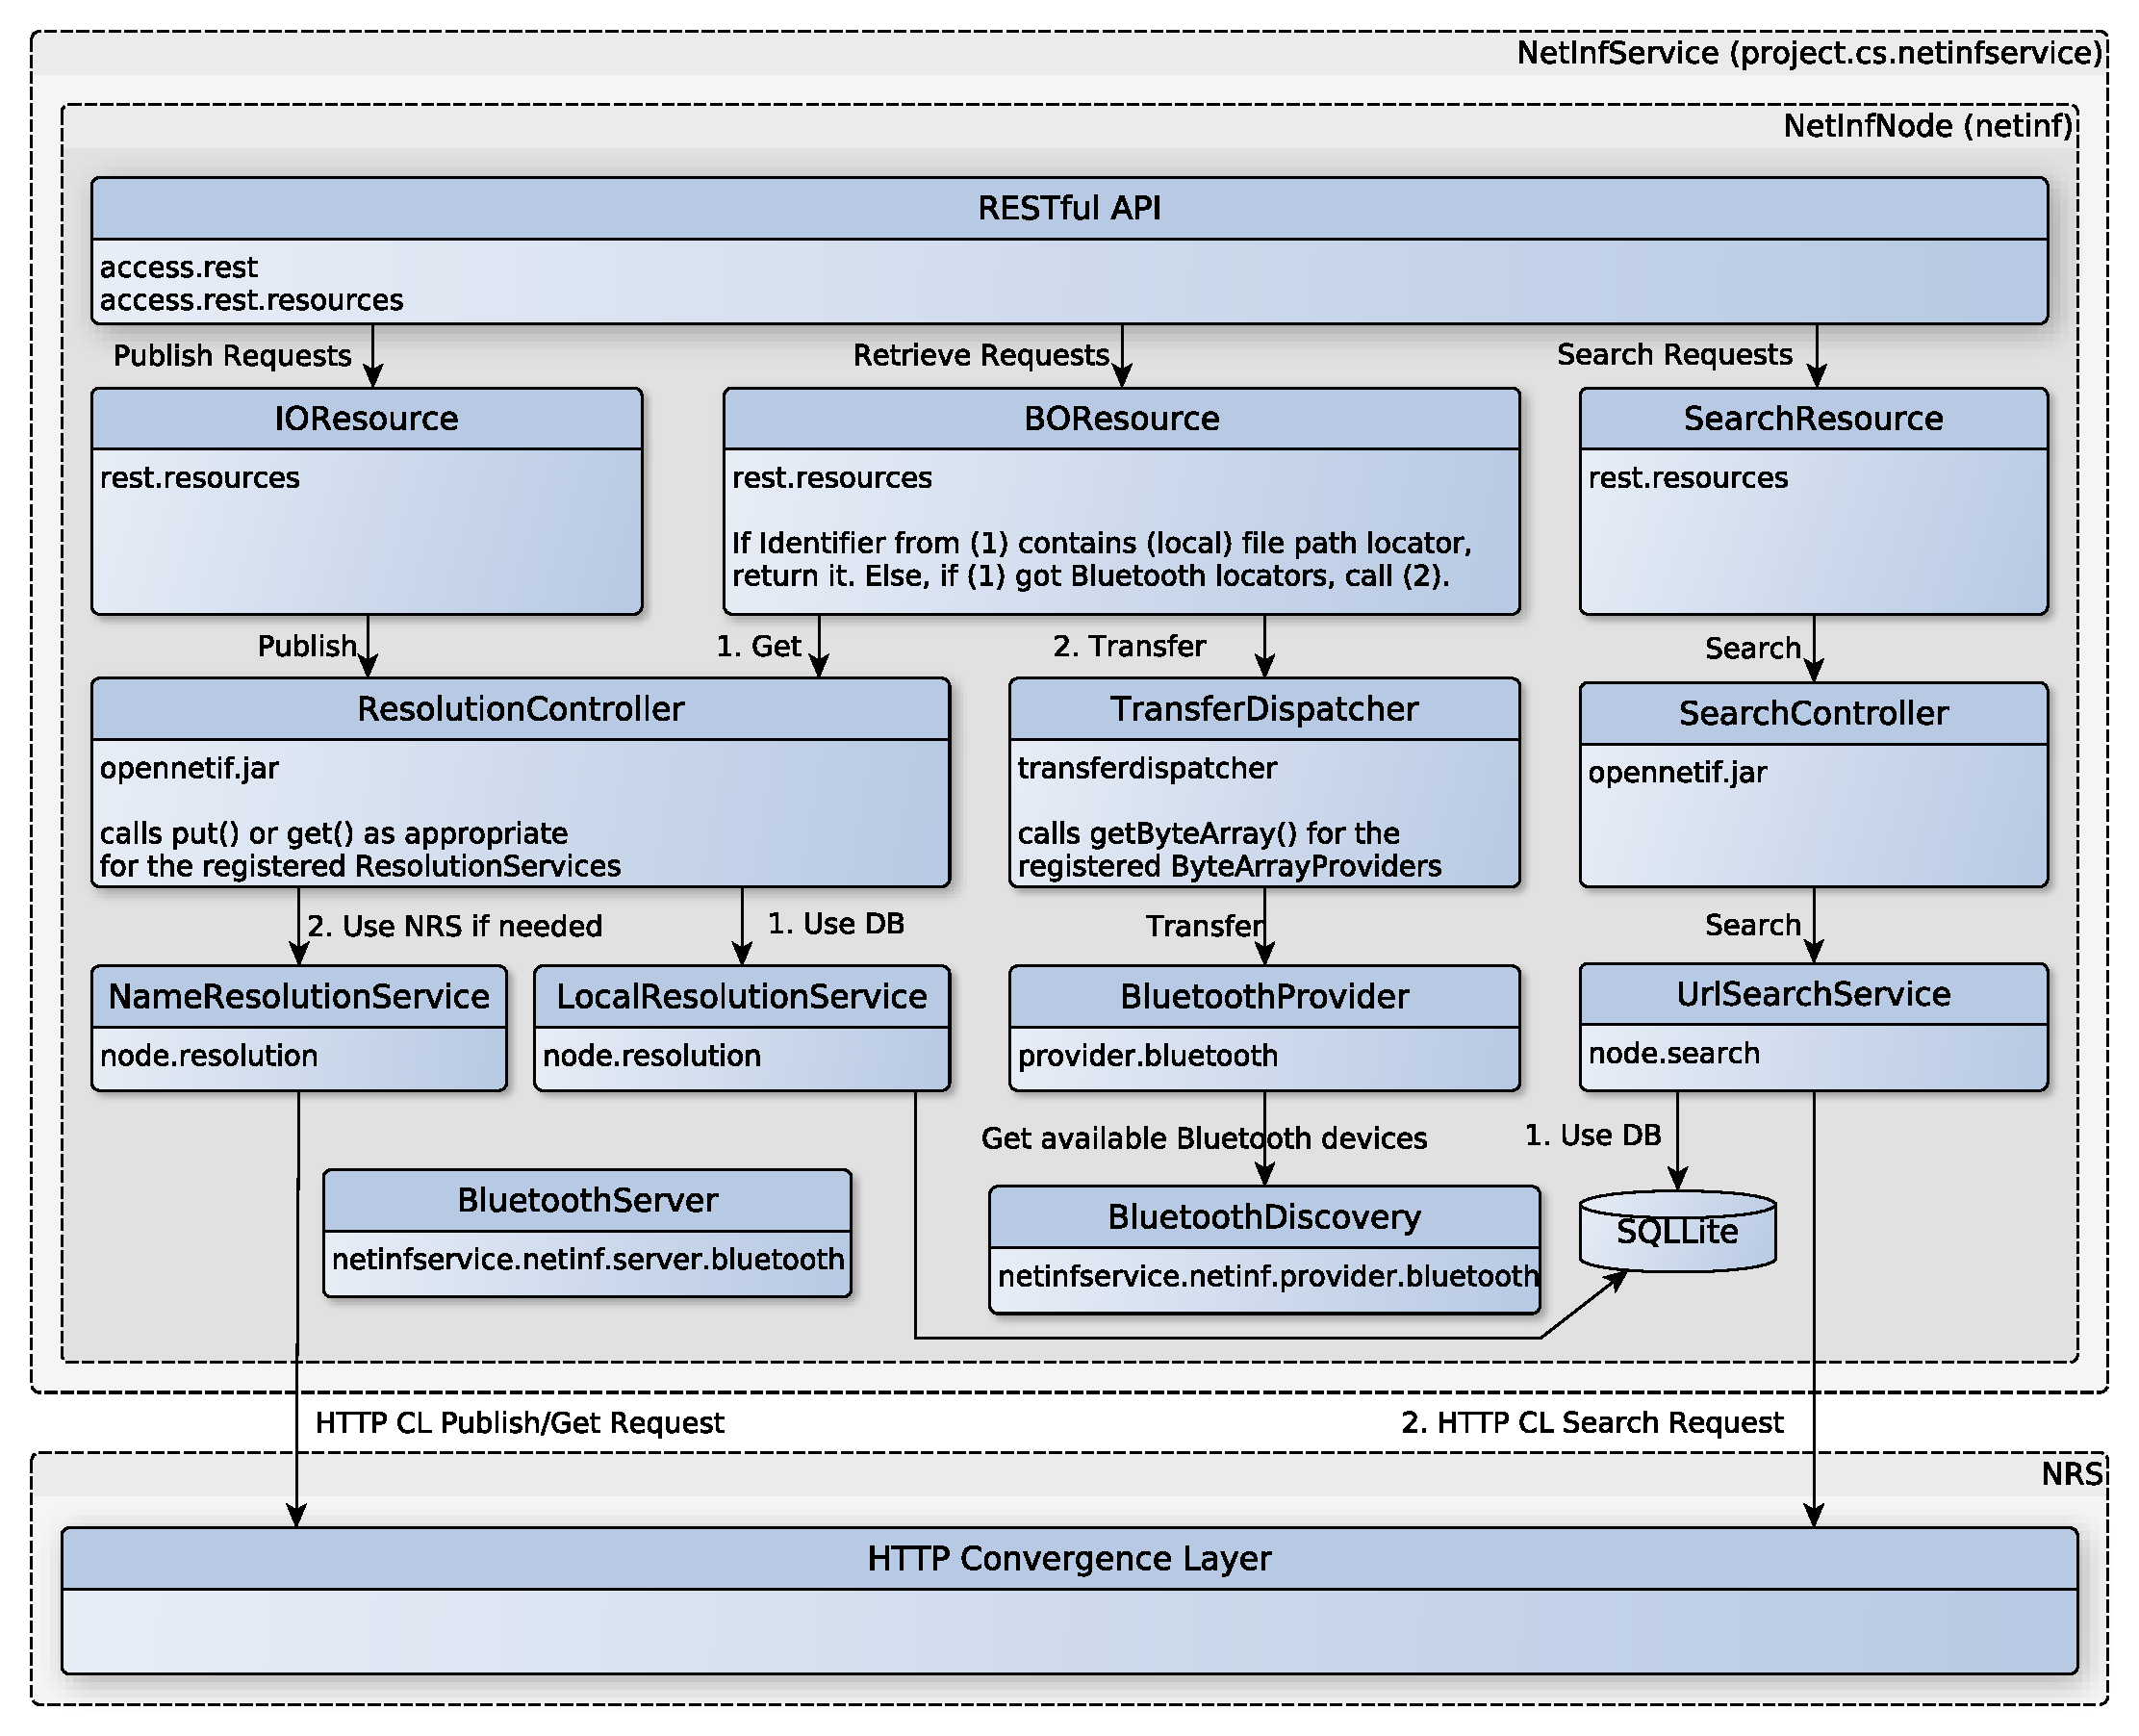
\includegraphics[width=1.4\textwidth]{./img/flowchart-NetInf.pdf}}
\caption{NetInfService Control Flow}
\label{fig:netinf-controlflow}
\end{figure}

\subsection{RESTful API Access}

Access to the RESTful API is handled by the subclasses of NetInfRequest. There are three subclasses NetInfPublish, NetInfRetrieve and NetInfSearch corresponding to the API calls for publish, retrieve and search. NetInfRequest extends the class AsyncTask provided by Android, and hence all subclasses of NetInfRequest are also AsyncTasks.

These classes can be used in two ways. Either by doing a blocking call:

\begin{code}[language=Java]
	// Create a new search
	NetInfSearch search = new NetInfSearch("tokens", "ext");
	// Execute the search
	search.execute();
	// Block until the search response is available
	NetInfSearchResponse searchResponse =
	        (NetInfSearchResponse) search.get();
	// Do things with the response...
\end{code}

Or in a non-blocking way by overriding the function that is called when the response becomes available:

\begin{code}[language=Java]
	// Create a new search
	NetInfSearch search = new NetInfSearch("tokens", "ext") {
            @Override
            public void onPostExecute(NetInfResponse response) {
                NetInfSearchResponse searchResponse =
                        (NetInfSearchResponse) response;
				// Do things with the response...
            }
    }
    // Execute the search
	search.execute();
\end{code}
